\documentclass{standalone}
\usepackage{tikz}
\usetikzlibrary{patterns, positioning}
\usepackage[sfdefault]{ClearSans} %% option 'sfdefault' activates Clear Sans as the default text font
\usepackage[T1]{fontenc}

\begin{document}
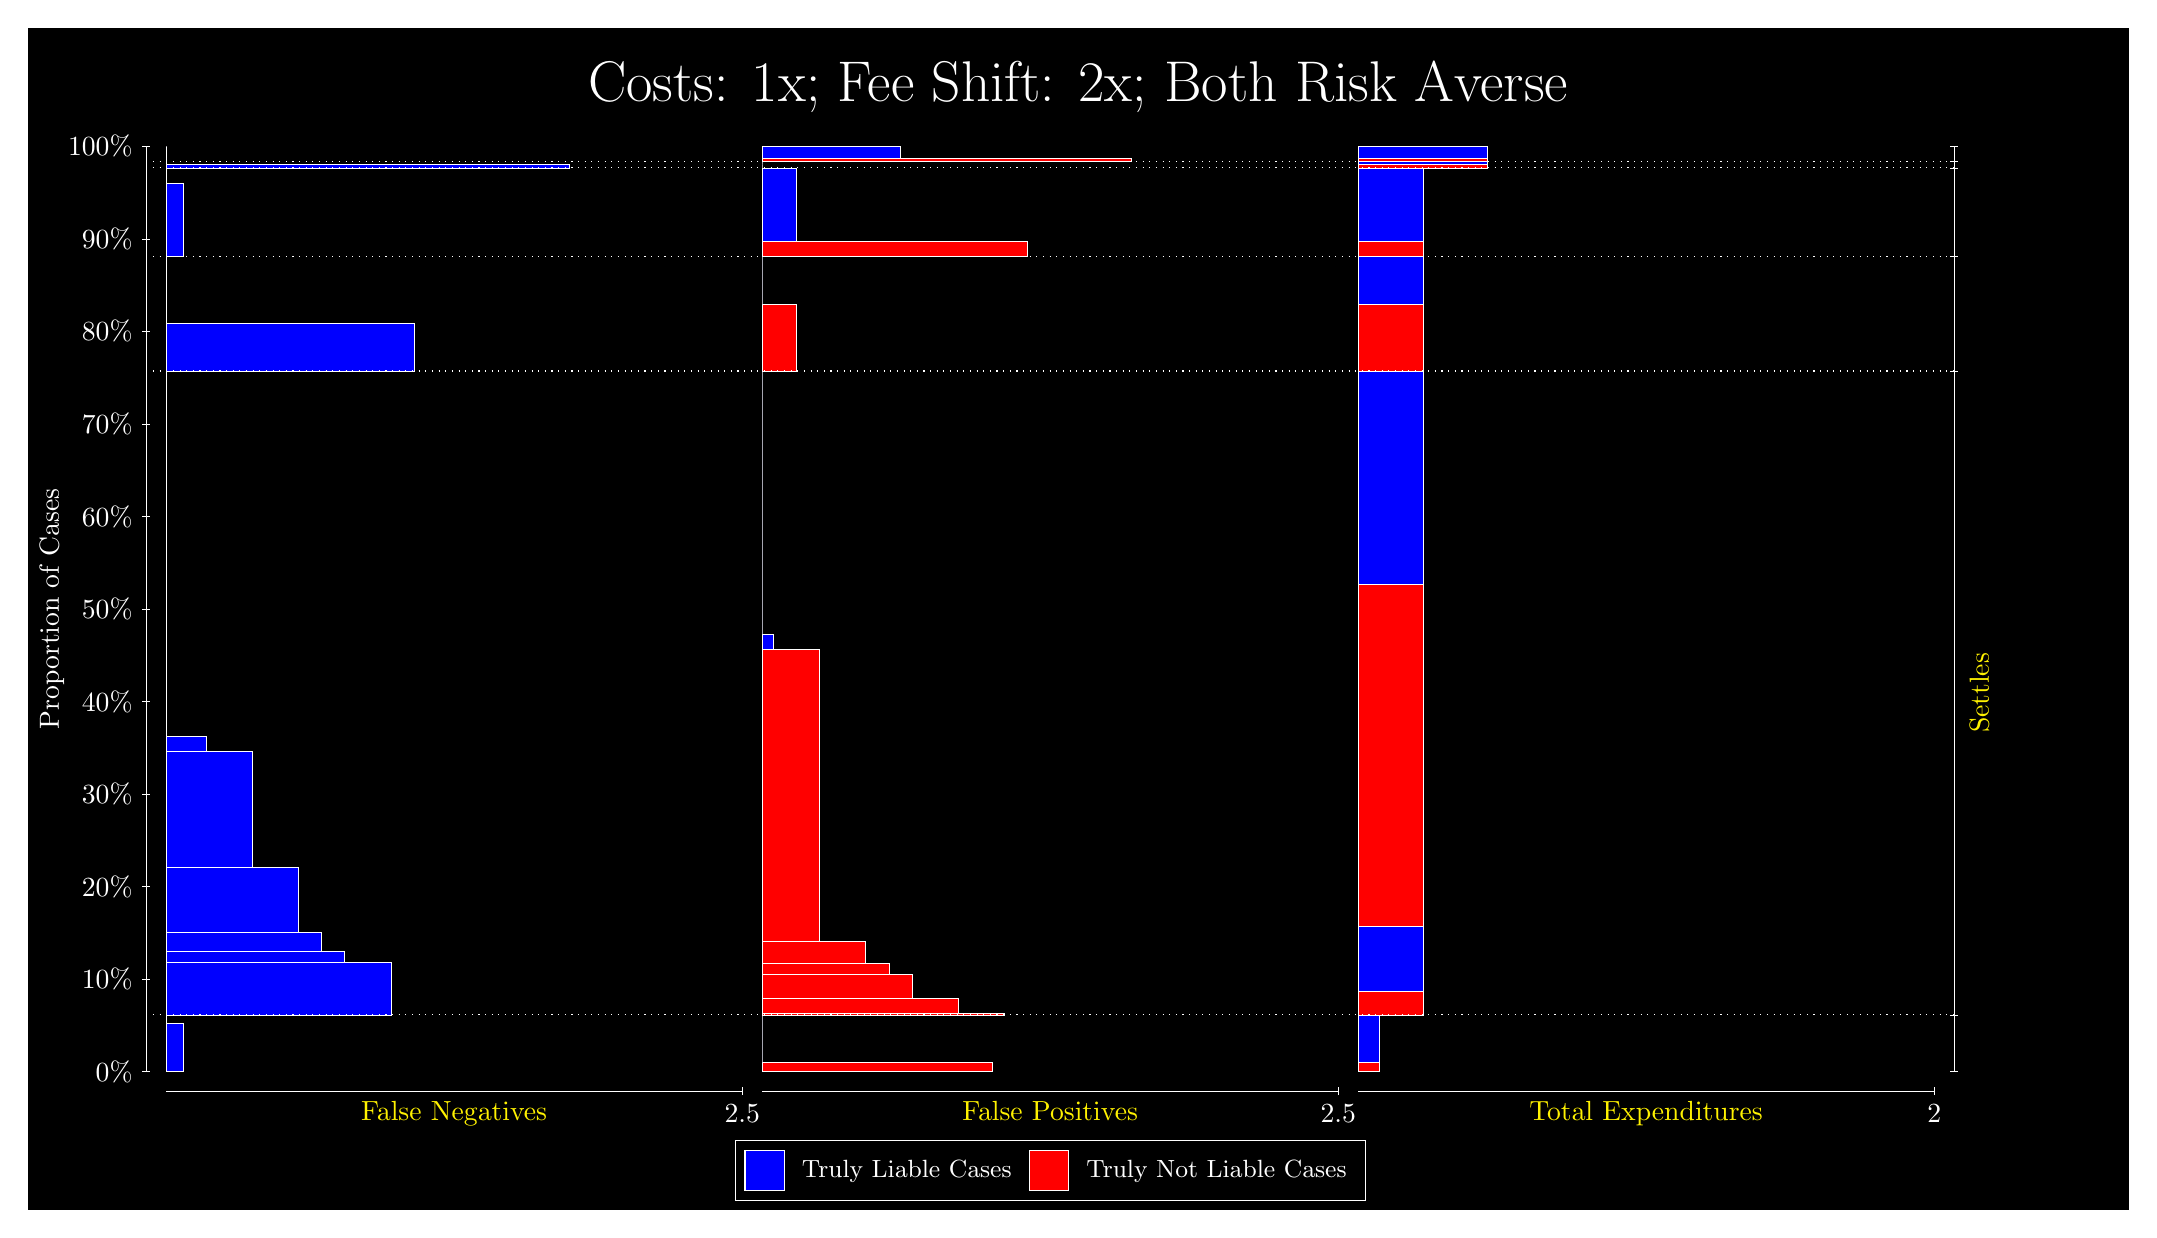
\begin{tikzpicture}
\draw[fill=black] (0,0) rectangle (26.667,15);
\draw[text=white] (0,13.5) rectangle (26.667,15) node[midway] {\huge Costs: 1x; Fee Shift: 2x; Both Risk Averse};
\draw[white, very thin] (1.5,1.75) -- (1.5,13.5);
\node[rotate=90, text=white, anchor=center] at (0.3, 7.625) {Proportion of Cases};
\draw[white, very thin] (1.45,1.75) -- (1.55,1.75);
\node[text=white, anchor=east] at (1.45, 1.75) {0\%};
\draw[white, very thin] (1.45,2.925) -- (1.55,2.925);
\node[text=white, anchor=east] at (1.45, 2.925) {10\%};
\draw[white, very thin] (1.45,4.1) -- (1.55,4.1);
\node[text=white, anchor=east] at (1.45, 4.1) {20\%};
\draw[white, very thin] (1.45,5.275) -- (1.55,5.275);
\node[text=white, anchor=east] at (1.45, 5.275) {30\%};
\draw[white, very thin] (1.45,6.45) -- (1.55,6.45);
\node[text=white, anchor=east] at (1.45, 6.45) {40\%};
\draw[white, very thin] (1.45,7.625) -- (1.55,7.625);
\node[text=white, anchor=east] at (1.45, 7.625) {50\%};
\draw[white, very thin] (1.45,8.8) -- (1.55,8.8);
\node[text=white, anchor=east] at (1.45, 8.8) {60\%};
\draw[white, very thin] (1.45,9.975) -- (1.55,9.975);
\node[text=white, anchor=east] at (1.45, 9.975) {70\%};
\draw[white, very thin] (1.45,11.15) -- (1.55,11.15);
\node[text=white, anchor=east] at (1.45, 11.15) {80\%};
\draw[white, very thin] (1.45,12.325) -- (1.55,12.325);
\node[text=white, anchor=east] at (1.45, 12.325) {90\%};
\draw[white, very thin] (1.45,13.5) -- (1.55,13.5);
\node[text=white, anchor=east] at (1.45, 13.5) {100\%};

\draw[white, very thin] (24.457,1.75) -- (24.457,13.5);
\draw[white, very thin] (24.407,1.75) -- (24.507,1.75);
\node[anchor=west] at (24.407, 1.75) {};
\draw[white, very thin] (24.407,2.4702) -- (24.507,2.4702);
\node[anchor=west] at (24.407, 2.4702) {};
\draw[white, very thin] (24.407,10.647) -- (24.507,10.647);
\node[anchor=west] at (24.407, 10.647) {};
\draw[white, very thin] (24.407,12.099) -- (24.507,12.099);
\node[anchor=west] at (24.407, 12.099) {};
\draw[white, very thin] (24.407,13.227) -- (24.507,13.227);
\node[anchor=west] at (24.407, 13.227) {};
\draw[white, very thin] (24.407,13.311) -- (24.507,13.311);
\node[anchor=west] at (24.407, 13.311) {};
\draw[white, very thin] (24.407,13.5) -- (24.507,13.5);
\node[anchor=west] at (24.407, 13.5) {};

\draw[white, very thin, fill=blue] (1.75,1.75) rectangle (1.9696,2.3589);
\draw[white, very thin, fill=red] (1.75,2.3589) rectangle (1.75,2.4702);
\draw[white, very thin, fill=blue] (1.75,2.4702) rectangle (4.6044,3.1319);
\draw[white, very thin, fill=blue] (1.75,3.1319) rectangle (4.0188,3.2761);
\draw[white, very thin, fill=blue] (1.75,3.2761) rectangle (3.7261,3.5199);
\draw[white, very thin, fill=blue] (1.75,3.5199) rectangle (3.4333,4.3439);
\draw[white, very thin, fill=blue] (1.75,4.3439) rectangle (2.8478,5.8159);
\draw[white, very thin, fill=blue] (1.75,5.8159) rectangle (2.2623,6.0034);
\draw[white, very thin, fill=red] (1.75,6.0034) rectangle (1.75,10.647);
\draw[white, very thin, fill=blue] (1.75,10.647) rectangle (4.8971,11.256);
\draw[white, very thin, fill=red] (1.75,11.256) rectangle (1.75,12.099);
\draw[white, very thin, fill=blue] (1.75,12.099) rectangle (1.9696,13.034);
\draw[white, very thin, fill=red] (1.75,13.034) rectangle (1.75,13.227);
\draw[white, very thin, fill=blue] (1.75,13.227) rectangle (6.8732,13.267);
\draw[white, very thin, fill=red] (1.75,13.267) rectangle (1.75,13.311);
\draw[white, very thin, fill=red] (1.75,13.311) rectangle (1.75,13.351);
\draw[white, very thin, fill=blue] (1.75,13.351) rectangle (1.75,13.5);
\draw[white, very thin, fill=red] (9.3189,1.75) rectangle (12.246,1.8613);
\draw[white, very thin, fill=blue] (9.3189,1.8613) rectangle (9.3189,2.4702);
\draw[white, very thin, fill=red] (9.3189,2.4702) rectangle (12.393,2.4836);
\draw[white, very thin, fill=red] (9.3189,2.4836) rectangle (11.807,2.6863);
\draw[white, very thin, fill=red] (9.3189,2.6863) rectangle (11.222,2.9848);
\draw[white, very thin, fill=red] (9.3189,2.9848) rectangle (10.929,3.1276);
\draw[white, very thin, fill=red] (9.3189,3.1276) rectangle (10.636,3.404);
\draw[white, very thin, fill=red] (9.3189,3.404) rectangle (10.051,7.1135);
\draw[white, very thin, fill=blue] (9.3189,7.1135) rectangle (9.4652,7.301);
\draw[white, very thin, fill=blue] (9.3189,7.301) rectangle (9.3189,10.647);
\draw[white, very thin, fill=red] (9.3189,10.647) rectangle (9.758,11.49);
\draw[white, very thin, fill=blue] (9.3189,11.49) rectangle (9.3189,12.099);
\draw[white, very thin, fill=red] (9.3189,12.099) rectangle (12.686,12.292);
\draw[white, very thin, fill=blue] (9.3189,12.292) rectangle (9.758,13.227);
\draw[white, very thin, fill=red] (9.3189,13.227) rectangle (9.3189,13.271);
\draw[white, very thin, fill=blue] (9.3189,13.271) rectangle (9.3189,13.311);
\draw[white, very thin, fill=red] (9.3189,13.311) rectangle (14.003,13.351);
\draw[white, very thin, fill=blue] (9.3189,13.351) rectangle (11.075,13.5);
\draw[white, very thin, fill=red] (16.888,1.75) rectangle (17.162,1.8613);
\draw[white, very thin, fill=blue] (16.888,1.8613) rectangle (17.162,2.4702);
\draw[white, very thin, fill=red] (16.888,2.4702) rectangle (17.711,2.7687);
\draw[white, very thin, fill=blue] (16.888,2.7687) rectangle (17.711,3.5927);
\draw[white, very thin, fill=red] (16.888,3.5927) rectangle (17.711,7.9375);
\draw[white, very thin, fill=blue] (16.888,7.9375) rectangle (17.711,10.647);
\draw[white, very thin, fill=red] (16.888,10.647) rectangle (17.711,11.49);
\draw[white, very thin, fill=blue] (16.888,11.49) rectangle (17.711,12.099);
\draw[white, very thin, fill=red] (16.888,12.099) rectangle (17.711,12.292);
\draw[white, very thin, fill=blue] (16.888,12.292) rectangle (17.711,13.227);
\draw[white, very thin, fill=red] (16.888,13.227) rectangle (18.534,13.271);
\draw[white, very thin, fill=blue] (16.888,13.271) rectangle (18.534,13.311);
\draw[white, very thin, fill=red] (16.888,13.311) rectangle (18.534,13.351);
\draw[white, very thin, fill=blue] (16.888,13.351) rectangle (18.534,13.5);
\draw[white, dotted] (1.5,2.4702) -- (24.457,2.4702);
\draw[white, dotted] (1.5,10.647) -- (24.457,10.647);
\draw[white, dotted] (1.5,12.099) -- (24.457,12.099);
\draw[white, dotted] (1.5,13.227) -- (24.457,13.227);
\draw[white, dotted] (1.5,13.311) -- (24.457,13.311);
\draw[white, very thin] (1.75,1.5) -- (9.0689,1.5);
\node[text=yellow, anchor=north] at (5.4094, 1.5) {False Negatives};
\draw[white, very thin] (9.0689,1.45) -- (9.0689,1.55);
\node[text=white, anchor=north] at (9.0689, 1.45) {2.5};

\draw[white, very thin] (9.3189,1.5) -- (16.638,1.5);
\node[text=yellow, anchor=north] at (12.978, 1.5) {False Positives};
\draw[white, very thin] (16.638,1.45) -- (16.638,1.55);
\node[text=white, anchor=north] at (16.638, 1.45) {2.5};

\draw[white, very thin] (16.888,1.5) -- (24.207,1.5);
\node[text=yellow, anchor=north] at (20.547, 1.5) {Total Expenditures};
\draw[white, very thin] (24.207,1.45) -- (24.207,1.55);
\node[text=white, anchor=north] at (24.207, 1.45) {2};


\node[text=yellow, centered, rotate=90] at (24.777, 6.5585) {Settles};





\draw (12.978300999999998,1.5) node[draw=none] (baseCoordinate) {};
\begin{scope}[align=center]
        \matrix[scale=0.5, draw=white, below=0.5cm of baseCoordinate, nodes={draw}, column sep=0.1cm]{
            \node[rectangle, draw, minimum width=0.5cm, minimum height=0.5cm, fill=blue] {}; &
            \node[draw=none, font=\small, text=white] (B) {Truly Liable Cases}; &
            \node[rectangle, draw, minimum width=0.5cm, minimum height=0.5cm, fill=red] {}; &
            \node[draw=none, font=\small, text=white] (B) {Truly Not Liable Cases}; \\
            };
\end{scope}

\end{tikzpicture}
\end{document}